\chapter{Building a Decentralized Application}\label{chapter:building-dapp}

\section{Introduction}
Chapter~\ref{chapter::app-concepts-design} focused on different application concepts and showed the underlying architecture for building decentralized applications where users are in control of their data. This chapter uses the concepts learned in the previous chapter to build two \textit{proof-of-concept} applications for secure file sharing. It will help us analyze the current \textit{state-of-the-art} protocols for building decentralized applications.

\section{Problem Context}
Existing applications for sharing files are central solutions and therefore suffer from a single point of failure risk. Moreover, using central services for securing data means that we have to trust a 3rd party with our data, thus exposing it to manipulation risks. Hence, a decentralized application is required to overcome the problems posed by a central application. With the recent developments in Blockchain technology and p2p storage, it is possible to securely store and share data without using any central server.

\section{Requirements}\label{sec:requirements}
A decentralized file sharing application should have following desirable properties:
\begin{itemize}
	\item Client-side encryption.
	\item Encryption keys are in the user's possession.
	\item Users can choose the data storage location.
	\item Easy and secure sharing of files with other users of the application.
\end{itemize}

\section{A File Sharing Application using Ethereum}
This section describes the workings of the application \textit{dShare-ethereum}\cite{harsh_kedia_2019_3359852} built using p2p technologies, enabling a secure way of storing and sharing data between two individuals or entities. The latest version of the application is deployed at \url{https://file-share-dapp.herokuapp.com/}

\subsection{Use Case}
Today's supply chain spans multiple geographies, but the documents involved in the industry, such as delivery certificates, are still in physical form. This paperwork prevents manipulations but leads to various delays across the whole chain, thus affecting everyone involved\cite{ibm:sc:1}.

The above problem can be solved by digitizing all documents, timestamping them using a trusted Time stamping authority (TSA) and upload them to a cloud service. However, the tools used to accomplish this solution are central services, and, therefore, suffers from data manipulations by a 3rd party.

We, therefore, need a solution that is peer-to-peer and decentralized. Modern distributed technologies offer a means of decentralized time stamping and enable peer-to-peer storage systems that are resistant to manipulations by any 3rd party.

\textit{dShare-ethereum} is built using decentralized technologies such as Bitcoin\cite{nakamoto2008bitcoin}, Ethereum\cite{buterin2014ethereum} and IPFS\cite{benet2014ipfs} such that it's capable of immutable timestamping and secure file sharing in a p2p fashion.

\subsection{Technologies Used}
\subsubsection{Ethereum}
Ethereum\cite{buterin2014ethereum} is a blockchain platform for building decentralized applications. It allows the creation of \textit{Smart Contracts}, which serves as a backend for the application. Solidity\cite{github:solidity:1} is the primary language for writing smart contracts on Ethereum.

\subsubsection{InterPlanetary File System (IPFS)}
IPFS is used as a decentralized storage for storing files and their corresponding decryption key, which are encrypted using the uploader's public key.

\subsubsection{OriginStamp}\label{sec:originstamp}
OriginStamp\cite{hepp2018originstamp} is a blockchain-based system for decentralized timestamping. It uses the Bitcoin blockchain for the creation of trusted and immutable timestamps for any piece of data. Timestamps created by OriginStamp can be verified independently by anyone.

\begin{figure}[h]
	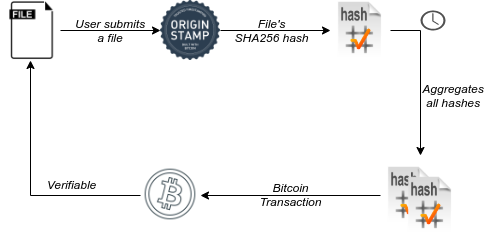
\includegraphics[width=\linewidth]{figures/origin-stamp}
	\caption{\label{fig:originstamp} Timestamping using OriginStamp}
\end{figure}

Figure~\ref{fig:originstamp} visualizes the timestamping process as implemented in OriginStamp. When a user submits a file, the hash of the data is recorded. It combines all the hashes submitted over a period of time and generates an aggregated hash. After some additional hashing and encoding operations, a Bitcoin address is created to which the smallest possible transactional amount of Bitcoins is transferred. Performing this transaction embeds the hash and the timestamp permanently to the Bitcoin blockchain. Each transaction is part of a block and is added to the Bitcoin blockchain by a process called mining. Since each block is linked cryptographically to the previous block, adding a new block confirms the validity of the last block. Changing the timestamp of a transaction becomes impossible once five or six subsequent blocks are mined, which requires an hour on average\cite{nakamoto2008bitcoin}.

\subsubsection{Firebase}
Firebase\cite{web:firebase:1} is used as a database for storing user's public keys, which is used for encryption of a file's key when it is shared with another user.

\subsubsection{MetaMask}
MetaMask\cite{web:metamask:1} is an Ethereum wallet. It serves as a web3\cite{web:web3:1} provider allowing any application to interact with the Ethereum blockchain.

\subsection{Application Architecture}

\begin{figure}[h]
	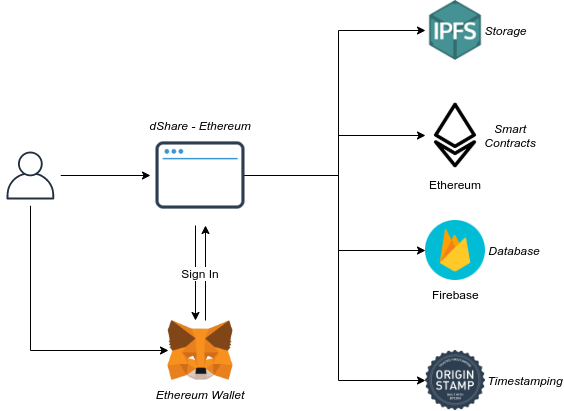
\includegraphics[width=\linewidth]{figures/dshare-ethereum}
	\caption{\label{fig:dshare-ethereum} \textit{dShare-ethereum} Architecture}
\end{figure}

Figure~\ref{fig:dshare-ethereum} visualizes the application architecture. MetaMask handles user authentication. For storing files, we use IPFS. Before uploading to the IPFS network, files are encrypted using AES-GCM\cite{web:aesgcm:1} encryption mechanism. Sharing of encryption keys is facilitated using smart contracts built on Ethereum; thus, files can be shared by anyone with an Ethereum address. Finally, OriginStamp is used for immutable timestamping.

The front-end of the application is built using React.js\cite{web:react:1}, a JavaScript library for building user interfaces. Solidity was used for writing smart contracts and deployed on the Ethereum test network, Rinkeby\cite{web:rinkeby:1}. Next.js\cite{web:next:1} was used for server-side rendering (SSR), and Firebase was used as a database for storing public Ethereum key of the users.

\subsection{Workings}
\subsubsection{Authentication}
When a user logs into the application, she is presented with a MetaMask dialog, which asks her to sign a randomly generated value. This signature is used to retrieve the public key for the selected Ethereum address. The public key is then saved to the database, and the user is logged in.

\subsubsection{Smart Contract}
The smart contract serves as the bridge between the front-end of the application and the Ethereum Blockchain. Data is read from and written to the blockchain with the help of function calls in the contract. Each function call that modifies some data requires a small fee in the form of gas\cite{se:answer:1} which defines the cost for a function execution in Ether. Reading from the blockchain does not require any fees.

The application makes use of two contracts, \textit{FileFactory}, which acts as the factory contract for the creation of new files and \textit{File}, which represents an individual file. Code for both the contracts is available at \url{https://github.com/hKedia/dShare/blob/master/ethereum/contracts/FileShare.sol}

\paragraph{FileFactory}
\textit{FileFactory} is the contract that is deployed on the Rinkeby test network. It has several mappings which store the list of file contracts uploaded by a user. Whenever a user uploads a file, a function call is made to the \textit{FileFactory} contract, which in turn deploys the \textit{File} contract and updates the mappings for list of uploaded files and the respective uploader.

\paragraph{File}
The \textit{File} contract is deployed to the blockchain whenever a file is successfully uploaded to the IPFS network using the application. Ones deployed, the constructor function is called. It takes the values passed by the \textit{FileFactory} contract and saves the details to it’s \textit{File} contract.

\subsubsection{File Upload}
Figure~\ref{fig:ethereum-upload} visualizes the working of the application when a user uploads a file. Reference code is available at \url{https://github.com/hKedia/dShare/blob/master/pages/files/upload.js}

\begin{figure}[h]
	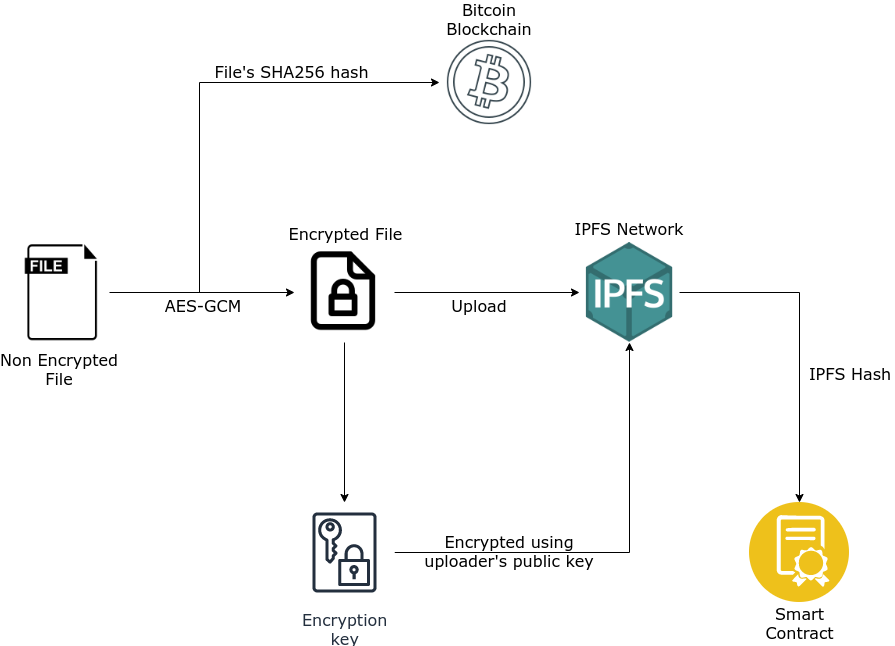
\includegraphics[width=\linewidth]{figures/ethereum-upload}
	\caption{\label{fig:ethereum-upload} File Upload using \textit{dshare-ethereum}}
\end{figure}

As soon as a user submits a file to be uploaded, it's SHA-256\cite{web:sha256:1} hash is calculated, and a timestamp is created by submitting the hash to the bitcoin blockchain using the OriginStamp API\cite{web:osdoc:1}.

Next, the file is encrypted using the SubtleCrypto\cite{web:subcrypto:1} interface with `AES-GCM' as the encryption algorithm. The encrypted data is then combined with the random salt to generate a \texttt{Uint8Array} buffer ready to be uploaded to the IPFS network.

The key used to encrypt the file is converted to \texttt{JSON} web key (jwk) format and is encrypted using the uploader's Ethereum public key, which is retrieved from the database. This encrypted key and the encrypted data is then uploaded to the IPFS network. Once the file is successfully uploaded, \texttt{createFile()} in the \texttt{FileFactory} contract is called which deploys a new \texttt{File} contract with all details regarding the file saved to the blockchain.

\subsubsection{File Sharing}
Sharing a file requires the recipient's Ethereum address and uploader's private key. Figure~\ref{fig:ethereum-share} visualizes the working of the application when a user shares a file with another user. Reference code is available at \url{https://github.com/hKedia/dShare/blob/master/components/FileSharing.js}

\begin{figure}[h]
	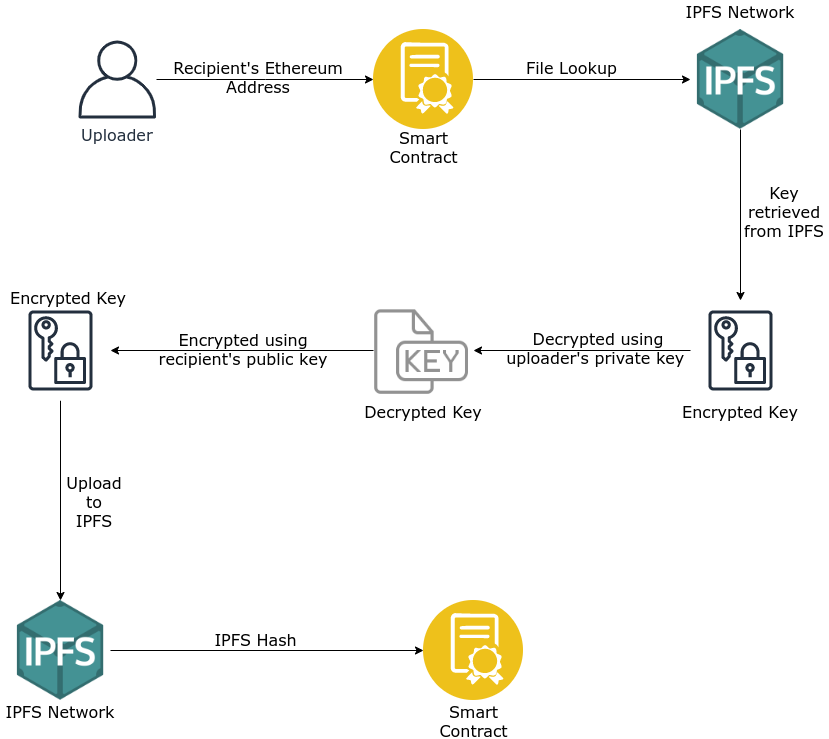
\includegraphics[width=\linewidth]{figures/ethereum-share}
	\caption{\label{fig:ethereum-share} File Sharing using \textit{dshare-ethereum}}
\end{figure}

Firstly, the file's IPFS location is retrieved from the \texttt{File} contract. From this location, the encrypted key is download and decrypted using uploader's private key. Once decrypted, the key is again encrypted using a recipient's public key. The new encrypted key is then uploaded to the IPFS network. Finally, the IPFS location of the key is saved into the \texttt{File} contract by calling \texttt{shareFile()}.

To stop sharing a file, a function call can be made to the \texttt{File} contract with the recipient's address, which deletes the contract reference from the \texttt{recipientFiles} array.

\subsubsection{File Download}
Downloading a file requires the user's Ethereum private key. Depending on whether the file is uploaded or shared one, the corresponding function from the \texttt{File} contract is called to retrieve the file's details. The key is then decrypted using user's private key and is converted to a valid JSON web key (jwk) \cite{rfc7517} format. The encrypted file data is then converted to a file buffer, and the original file content and the random salt used for encrypting the file is retrieved. Finally, the file is decrypted and saved to the user's local storage. Reference code for file download is available at \url{https://github.com/hKedia/dShare/blob/master/components/FileDownload.js}

\subsubsection{File Archiving}
Instead of deleting a \texttt{File} contract, the application provides a way to achieve files. This is also useful to keep track of archived files and restore them at a later date if required. When a file is archived, the \texttt{File} contract address is saved in an array, which is later used for filtering the archived files from the UI. Restoring a file removes the \texttt{File} contract address from the archived files array. The reference code for file archiving is available at \url{https://github.com/hKedia/dShare/blob/master/components/FileDetail.js#L71}

\subsection{Limitations}
This application is built using experimental p2p technologies that are changing very rapidly. Below are some of the limitations:

\begin{itemize}
	\item IPFS nodes treat the stored data as cache, meaning there is no guarantee the data will continue to be available. To overcome this, users should run their own IPFS nodes and \textit{pin}\cite{web:ipfs:pin:1} the important data.
	
	\item MetaMask, the Ethereum wallet used in the application has no function that allows us retrieve the private key of the user within the application. Therefore, whenever a user wants to share or download a file, the private key must be manually provided for decryption.
	
	\item Files can be only be shared with recipients who have logged into the application at least once.
\end{itemize}

\section{A File Sharing Application using Blockstack}
This section describes the workings of the application \textit{dshare-blockstack}\cite{harsh_kedia_2019_3359854} built using Blockstack\cite{blockstack2019whitepaper}, a decentralized computing network and app ecosystem. The latest version of the application is deployed at \url{https://dshare-blockstack.herokuapp.com/}.

\subsection{Use Case}
\textit{dshare-blockstack} focuses on the easy sharing of files between two users. The encryption and decryption are handled by keys generated on user's machine. It leverages the existing cloud infrastructure for storage, thereby providing rich user experience.

\subsection{Technologies Used}
\subsubsection{Blockstack}
Blockstack\cite{ali2016blockstack} is a platform for building highly scalable decentralized applications where users own their data. It implements a DPKI system (see Section~\ref{sec:blockstack-auth}) anchored on the Bitcoin blockchain. It also implements a storage system, Gaia (see Section~\ref{sec:blockstack-gaia}), which leverages the existing cloud infrastructure providing users with private data lockers.

\subsubsection{Radiks}
``Radiks\cite{github:radiks:server:1} is a framework for building complex and collaborative decentralized applications, using Blockstack infrastructure under the hood" \cite{web:radiks:1}. It serves as a indexing server for data that is stored in Gaia. \textit{dshare-blockstack} uses the front-end component library, \textit{radiks.js}\cite{github:radiksjs:1} for interacting with Radiks.

\subsection{Application Architecture}
\begin{figure}[h]
	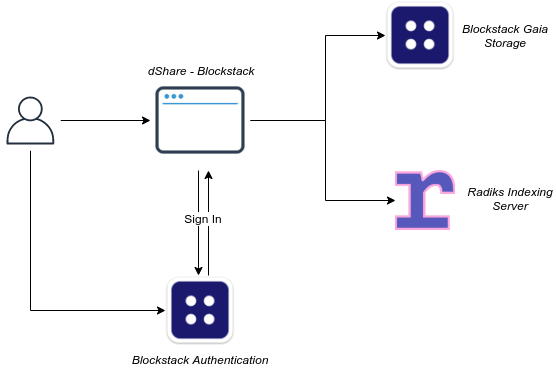
\includegraphics[width=\linewidth]{figures/dshare-blockstack}
	\caption{\label{fig:dshare-blockstack} \textit{dShare-blockstack} Architecture}
\end{figure}

Figure~\ref{fig:dshare-blockstack} visualizes the application architecture. User authentication is handled by the Blockstack Browser. Files are uploaded to the user's Gaia Hub, a private data locker in the cloud. Before uploading, files are encrypted using a symmetric key employing AES-GCM as the encryption mechanism. Sharing logic is implemented using Radiks, which provides an API for creating data models to represent uploaded files.

\subsection{Workings}

\subsubsection{Authentication}
When a user signs into the application, she is redirected to the Blockstack browser. Here she can create a new Blockstack ID or select one of her existing IDs. See Section~\ref{sec:blockstack-auth} for the authentication flow. Once authenticated, the user is redirected back to the application and logged in. The public key of the user is saved under \textit{/keys} inside her Gaia hub, which is later used for encrypting a file's encryption key.

\subsubsection{File Upload}
Figure~\ref{fig:blockstack-upload} visualizes the working of the application when a user uploads a file. The reference code for the functionality is available at \url{https://github.com/hKedia/dShare-blockstack/blob/master/pages/files/upload.js#L71}.

\begin{figure}[h]
	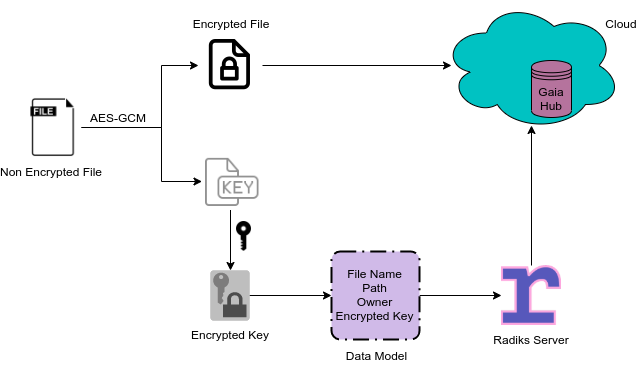
\includegraphics[width=\linewidth]{figures/blockstack-upload}
	\caption{\label{fig:blockstack-upload} File Upload using \textit{dShare-blockstack}}
\end{figure}

When a user submits a file to be uploaded, it gets encrypted using the SubtleCrypto interface with AES-GCM as the encryption algorithm. The encrypted data is combined with the random salt to generate a \texttt{Unit8Array} buffer. A unique \textit{identifier} is generated for the file path using the shortid\cite{github:shortid:1} library. The \texttt{Uint8Array} buffer is then uploaded to user's Gaia hub under `files/{\textit{identifier}}'.

The \textit{key} used to encrypt the file is first converted to JSON Web Token (JWT) \cite{rfc7519} format and then is encrypted using the user's public key. A data model is created, which includes the filename, path, owner, and the encrypted key. This data model is saved to the radiks server, which in turn saves the data to the Gaia hub.

\subsubsection{File Sharing}
Sharing a file requires the recipient's Blockstack ID. Figure~\ref{fig:blockstack-share} visualizes the working of the application when a user shares a file with another user. The reference code is available at \url{https://github.com/hKedia/dShare-blockstack/blob/master/pages/files/view.js#L93}.

\begin{figure}[h]
	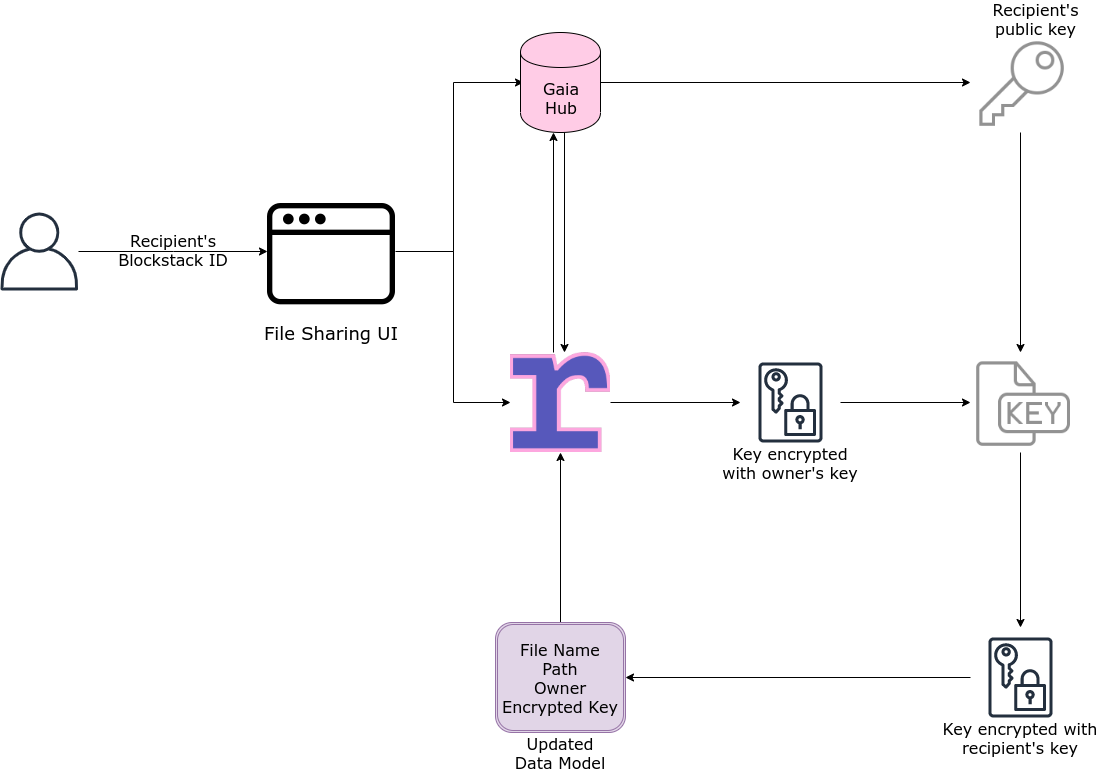
\includegraphics[width=\linewidth]{figures/blockstack-share}
	\caption{\label{fig:blockstack-share} File Sharing using \textit{dShare-blockstack}}
\end{figure}

Firstly, the recipient's public key is retrieved from the Gaia hub located under `\textit{keys/}'. The \textit{key} used to encrypt the file is downloaded and then decrypted using the user's private key. The decrypted key is then encrypted using the recipient's public key. The data model associated with the file is updated with the recipient Blockstack ID and the newly encrypted key is saved to the Radiks server. 

When the user stops sharing a file, the recipient ID and the associated encrypted key is removed from the data model associated with the file.

\subsubsection{File Download}
Downloading a file follows below steps:

\begin{itemize}
	\item Retrieve the data model associated with the current file.
	\item Get the file's name, path, owner, and the encryption key from the data model.
	\item Decrypt the encrypted \textit{key} using the user's private key.
	\item Retrieve the encrypted file content and convert it to a \texttt{Uint8Array} buffer.
	\item Separate the original file content and the random salt.
	\item Decrypt the file using the downloaded key and save the file to the user's device.
\end{itemize}

The reference code implementing file download is available at \url{https://github.com/hKedia/dShare-blockstack/blob/master/pages/files/view.js#L40}

\subsubsection{File Deletion}
Deleting a file involves destroying the data model associated with the file. Reference code is available at \url{https://github.com/hKedia/dShare-blockstack/blob/master/pages/files/view.js#L83}

\subsection{Limitations}
Below are some of the limitations of \textit{dShare-blockstack}:

\begin{itemize}
	\item To use the application, the user must use a Blockstack ID with an associated username.
	\item The application uses the default Gaia storage, which has a 25 MB file size limit.
	\item Files can only be shared with recipients who have logged into the application at least once.
\end{itemize}

\section{Related Work}
\subsection{Timestamping}
Trusted timestamping is a way of verifying that specific information existed at a given point in time. Blockchains enables anchoring of data utilizing cryptocurrency transactions where each transaction gets an immutable timestamp.

\subsubsection{Proof of Existence}
Proof of Existence\cite{web:poex:1} is a web-based service that implements the concept of immutable timestamping using the Bitcoin blockchain. It notarizes data in the blockchain by submitting the hash of the data in a Bitcoin transaction. Currently, the service requires 0.00025BTC for every certification, which makes it expensive to timestamp large volumes of data.

\subsubsection{Chainpoint}
Chainpoint\cite{web:chainpoint:1} works similarly to OriginStamp (see Section~\ref{sec:originstamp}). The service runs on the Tierion\cite{web:tierion:1} Network, providing a scalable protocol for anchoring data in a blockchain and generating blockchain receipts. These receipts are called chainpoint proofs, which defines a path of operations that cryptographically links the data to one or more blockchains.

\subsection{Storage}
P2P protocols such as BitTorrent\cite{cohen2008bittorrent}, Distributed Hash Tables (DHT), and Git allows us to store information distributed across multiple computers. Coupled with a Blockchain, it enables a decentralized storage market.

\subsubsection{Sia}
Sia\cite{vorick2014sia} is a decentralized cloud storage system that allows its users to rent storage among peers utilizing storage contracts, which are cryptographically secured by saving on a blockchain. This makes the storage contracts tamper-proof and publicly auditable.

To ensure that the storage provider holds a client's data at a given time, they continuously need to submit storage proofs. The network consensus allows automatic verification of storage proofs and enforcement of storage contracts. The availability of data is ensured using redundancy techniques such as erasure codes.

Sia uses a variant of Bitcoin blockchain for storing the contracts, and the user must use Siacoin, an ERC-20 token in order to transact on the Sia network.

\subsubsection{Storj}
Storj\cite{wilkinson2014storj} works similarly to Sia. It is built on Kademlia\cite{maymounkov2002kademlia} DHT, connecting peers who can transact with each other. A transaction can involve negotiation of storage contract, transfer of data, verifying remote data, downloading of data, or payments to other nodes. Each peer is capable of doing transactions independently without any human involvement.

Storj uses the Ethereum blockchain for managing its storage contracts. They are stored as a versioned data structure describing the relationship between a client and a storage provider. Users must use Storjcoin, an ERC-20 token, to perform transactions on the Storj network.

\subsection{Blockchain}
Bitcoin\cite{nakamoto2008bitcoin} and Ethereum\cite{buterin2014ethereum}, the two most popular public blockchains are based on \textit{proof-of-work} (PoW)\cite{wiki:pow} consensus algorithm. PoW blockchains require a large number of computing resources to achieve consensus. This computing power largely go wasted, making PoW blockchains non-scalable and expensive to use. \textit{Proof-of-stake} (PoS)\cite{wiki:pos} blockchains, on the other hand, does not depend on computing resources but rather require a stake in the participating blockchain. This makes PoS blockchains both scalable and inexpensive to use.

\subsubsection{Cardano}
Cardano\cite{web:cardano:1} is a \textit{proof-of-stake} blockchain employing a peer reviewed academic approach. It's consensus algorithm, \textit{Ouroboros}\cite{kiayias2017ouroboros} is provably secure with rigorous security guarantees. Cardano is a multi layered blockchain. \texttt{ADA}, the internal currency of Cardano lives on the settlement layer, while control layer will run smart contracts.

Smart contracts in Cardano are written in Plutus\cite{web:plutus:1}, a functional smart contract language based on Haskell. It also employs a domain-specific language (DSL), Marlowe\cite{seijas2018marlowe}, for writing financial contracts.

Cardano will also implement on-chain governance and a {treasury system}\cite{zhang2019treasury}, making it a highly sustainable public blockchain.